\chapter{Praktischer Teil}
\thispagestyle{fancy} % Manually set the page style
Im praktischen Teil dieser komplexen Leistung werden die in der Theorie erläuterten Konzepte angewendet und in ein Programm umgesetzt. \newline Da die Erklärung des gesamten Programms den Rahmen dieser Arbeit sprengen würde, wird hier nur auf die wichtigsten Aspekte eingegangen. Der Quellcode des Programms ist im Anhang zu finden. Der Quellcode ist an den wichtigen Stellen mit Kommentaren versehen.

\section{Benutzeroberfläche}
Das Programm \textit{Fraktale} ist ein interaktives Programm, um Fraktale zu
visualisieren und zu erkunden. \newline Es besteht aus zwei Teilen: Einer
Zeichenfläche, auf die Fraktale gerendert werden, und einem Einstellungsfenster,
in dem man das aktuelle Fraktal und dessen Parameter, wie die Anzahl der
Iterationen und den Farbgebungsalgorithmus, einstellen kann. Das Fraktal kann
man ganz einfach mit der Maus verschieben und mit dem Mausrad zoomen.

\begin{figure}[H]
    \centering
    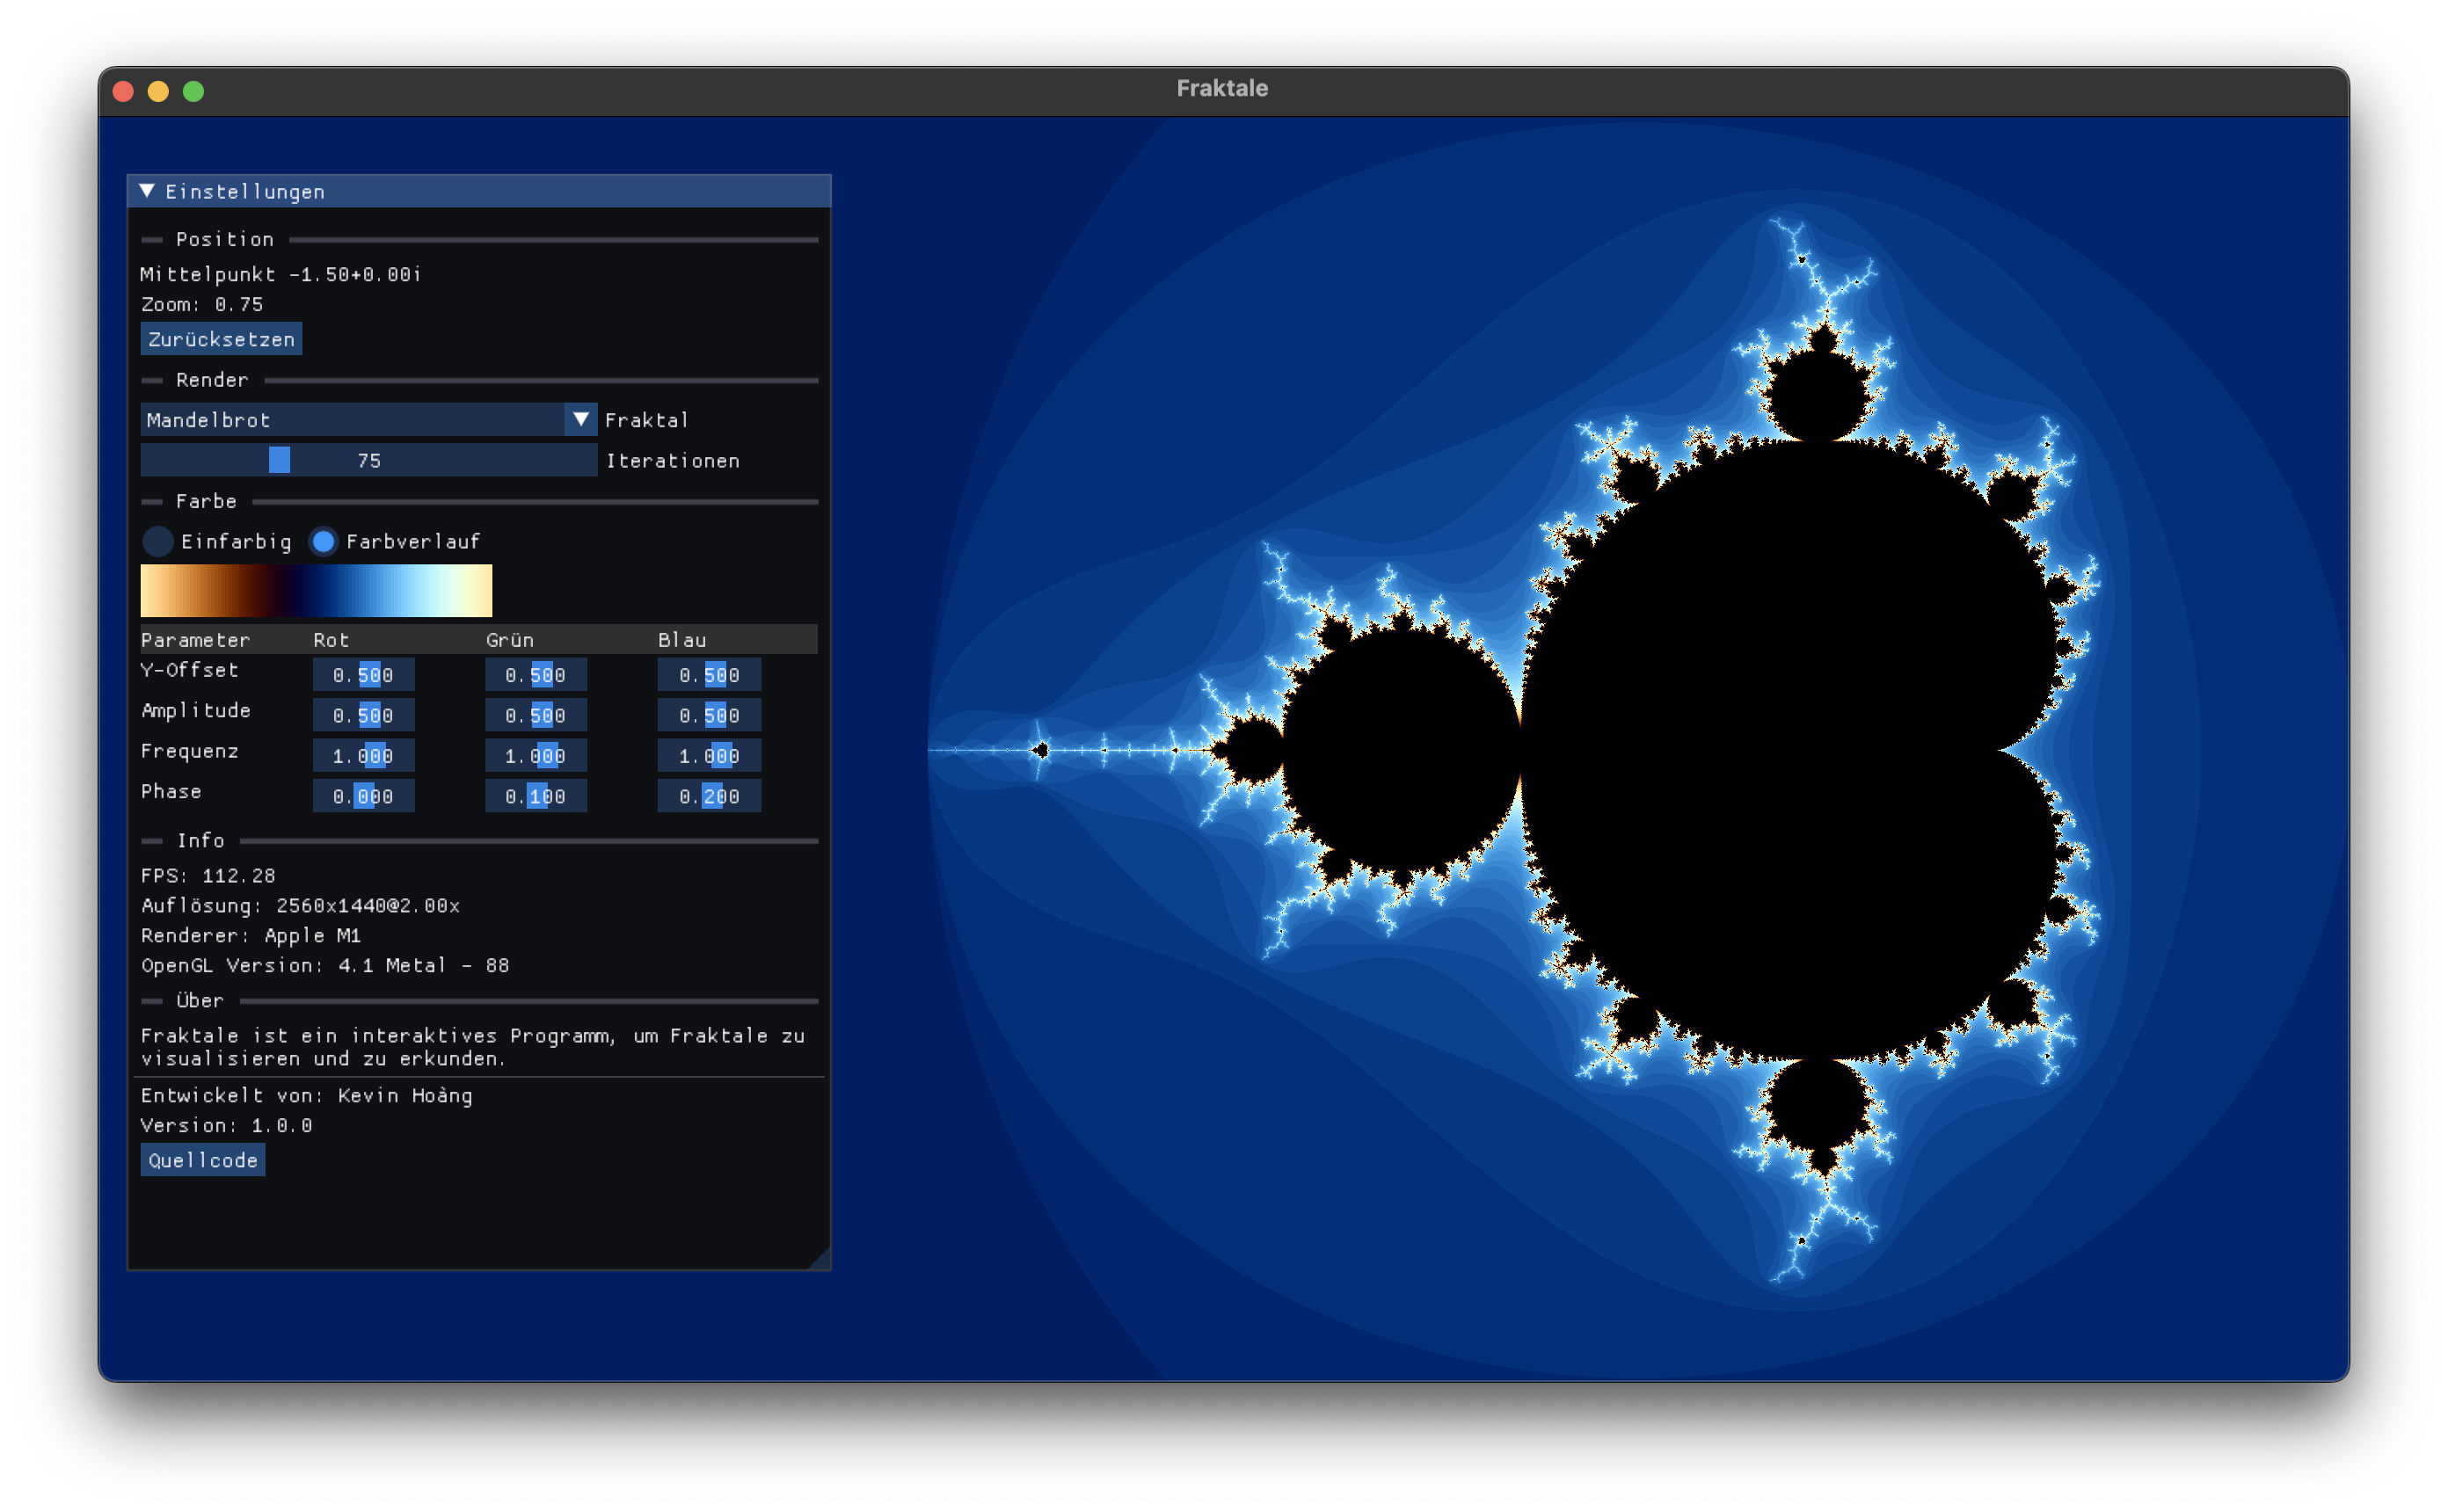
\includegraphics[width=0.8\textwidth]{img/Programm.png}
    \caption{Das Programm \textit{Fraktale}}
\end{figure}

\section{Programmaufbau}
Das Programm wurde in der Programmiersprache \textit{C++} geschrieben und nutzt
die Programmierschnittstelle \textit{OpenGL} um eine effiziente und
leistungsstarke Umsetzung der Algorithmen zu ermöglichen. Die Algorithmen
wurden in Form von \textit{Shadern} implementiert, die auf der Grafikkarte
ausgeführt werden. Diese werden in der Programmiersprache \textit{GLSL}
geschrieben.\hfill \break \newline \noindent Zusätzlich wurden Bibliotheken
verwendet, deren genauere Beschreibung und Funktion sich im Anhang befindet.
\hfill \break \newline \noindent Das Programm besteht aus folgenden Dateien:
\begin{itemize}
    \item \texttt{main.cpp} - Die Hauptdatei, in der das Programm initialisiert wird.
    \item \texttt{window.h} - In dieser Datei befinden sich Funktionen, die das Fenster erstellen und verwalten.
    \item \texttt{dearimgui.h} - In dieser Datei befinden sich Funktionen, um die Benutzeroberfläche zu erstellen und zu verwalten.
    \item \texttt{callbacks.h} - In dieser Datei befinden sich Funktionen, um die Fraktale mit der Maus zu verschieben und zu zoomen.
    \item \texttt{shader.h} / \texttt{shader.cpp} - Eine Hilfsdatei, die das Laden und Kompilieren von Shadern ermöglicht.
    \item \texttt{misc.h} - Hilfsdatei, die Funktionen enthält, die in anderen Dateien verwendet werden.
    \item \texttt{VertexShader.vert} - Der Vertex Shader, welcher für die Positionierung der \textit{Vertices} zuständig ist.
    \item \texttt{FragmentShader.frag} - Der Fragment Shader, wo die eigentliche Berechnung des Fraktals stattfindet.
\end{itemize}
\noindent
In der Datei \texttt{main.cpp} werden in der \texttt{main}-Funktion die
Funktionen zum Erstellen des Fensters und der grafischen Benutzeroberfläche
sowie OpenGL Funktionen aufgerufen. Die weitere Ausführung des Programms findet
in der \textit{Hauptschleife} statt, welche durch die Bedingung
\texttt{window\_should\_close()} gesteuert wird. In dieser Schleife werden die
C++ Variablen an den Shader übergeben, der \textit{Framebuffer} gerendert und
die grafische Benutzeroberfläche mittels \textit{Dear ImGui} gezeichnet.

\section{Implementierung der Algorithmen}
Die Algorithmen wurden in der Programmiersprache GLSL implementiert. In dieser
Programmiersprache gibt es die Datentypen \texttt{int} und \texttt{float} für
ganze und gebrochene Zahlen. Außerdem gibt es die Typen \texttt{vec2},
\texttt{vec3} und \texttt{vec4}, welche einen jeweils n-dimensionalen Vektor
repräsentieren. \newline Der GLSL Code des Shaders wird für jedes Pixel des
Framebuffers ausgeführt. Die Position des aktuellen Pixels ist durch die
Variable \texttt{gl\_FragCoord} gegeben. \newline Dieser Pixel wird zunächst in
eine komplexe Zahl umgewandelt, welches in der \texttt{map}-Funktion geschieht.
Mit den \textit{Uniform}-Variablen \texttt{u\_resolution}, \texttt{u\_offset}
und \texttt{u\_zoom} werden die Verschiebung und der Zoom unter
Berücksichtigung der Auflösung des Fensters berechnet. Dies ermöglicht es dem
Benutzer, das Fraktal mit der Maus zu verschieben und zu zoomen. \newline
\hfill \break \noindent Da es in GLSL keine komplexen Zahlen gibt, wird in der
Implementierung der Typ \texttt{vec2} verwendet, um eine komplexe Zahl $z=a+bi$
darzustellen, was zur folgenden Variablendeklaration führt:
\begin{verbatim}
    vec2 z = vec2(a, b);
\end{verbatim}

\subsection{Mandelbrot-Menge}
Die Mandelbrot-Menge wird in der Funktion \texttt{mandelbrot} berechnet. Diese
hat als Parameter eine komplexe Zahl \texttt{c} und gibt die Anzahl der
Iterationen \texttt{n} zurück, die benötigt werden, um festzustellen, ob die
komplexe Zahl \texttt{c} in der Mandelbrot-Menge liegt.
\begin{verbatim}
float mandelbrot(vec2 c) {
    vec2 z = vec2(0.0, 0.0);
    float n = 0.0;
    for(int i = 0; i < int(u_iterations); i++) {
        z = vec2(z.x * z.x - z.y * z.y, 2.0 * z.x * z.y);
        z += c;
        n += 1.0;
        if(length(z) > 2.0) {
            break;
        }
    }
    return n;
}
\end{verbatim}

\noindent
Um die iterative Vorschrift $z_{n+1} = z_n^2 + c$ zu implementieren, wird die
Variable \texttt{z} mit einem Startwert von 0 festgelegt. In der Schleife wird
die \texttt{z} zuerst quadriert und dann die komplexe Zahl \texttt{c} addiert.

%Die Berechnung des Quadrates von \texttt{z} erfolgt durch die Rechenregel für
%die Multiplikation komplexer Zahlen (siehe Theoretischer Teil).\newline 
\noindent
Die Bildung des Quadrates von \texttt{z} erfolgt durch Anwendung der 2.
binomischen Formel:
\begin{align*}
    z^2 & = (a+bi)^2             \\
    z^2 & = a^2 + 2abi - b^2     \\
    z^2 & = (a^2 - b^2) + (2ab)i
\end{align*}
Folglich in GLSL:
\texttt{z = vec2(z.x * z.x - z.y * z.y, 2.0 * z.x * z.y);}.
\hfill \break

\noindent
Die Addition komplexer Zahlen ist analog zur Addition von Vektoren: \texttt{z
    += c}. \hfill \break \newline Die Funktion \texttt{length} berechnet die Länge
eines Vektors, welche dem Betrag einer komplexen Zahl entspricht. Falls dieser
größer als 2 ist, wird die Schleife abgebrochen und die Anzahl der Iterationen
zurückgegeben. \newline Falls die Schleife nicht abgebrochen wird, wird die
Anzahl der maximal eingestellten Iterationen \texttt{u\_iterations}
zurückgegeben.

\subsection{Julia-Mengen}
Die Julia-Menge wird in der Funktion \texttt{julia} berechnet. Diese ist analog
zur Funktion \texttt{mandelbrot} aufgebaut, die komplexe Zahl \texttt{c} wird
hier jedoch als Startwert verwendet. Nach dem Quadrieren wird die komplexe Zahl
\texttt{u\_julia\_c} addiert, welche vom Benutzer eingestellt werden kann.
\begin{verbatim}
float julia(vec2 c) {
    vec2 z = c;
    float n = 0.0;
    for(int i = 0; i < int(u_iterations); i++) {
        z = vec2(z.x * z.x - z.y * z.y, 2.0 * z.x * z.y);
        z += u_julia_c;
        n += 1.0;
        if(length(z) > 2.0) {
            break;
        }
    }
    return n;
}
\end{verbatim}

\subsection{Farbgebung}
Nachdem man alle Punkte der Mandelbrot-Menge und der Julia-Menge berechnet hat,
kann man die zugehörigen schwarzen Bereiche einzeichnen. Punkte, die nicht
dazugehören, werden eingefärbt. Dies kann entweder einfarbig, mit verschiedenen
Helligkeitsstufen einer Farbe erfolgen, die je nach Anzahl der benötigten
Iterationen variiert, wenn der Betrag von $z$ gegen unendlich divergiert.
Alternativ kann auch eine Farbpalette verwendet werden, was zu interessanten
Abbildungen führt.

% \begin{figure}[H]
%     \minipage{0.45\textwidth}
%     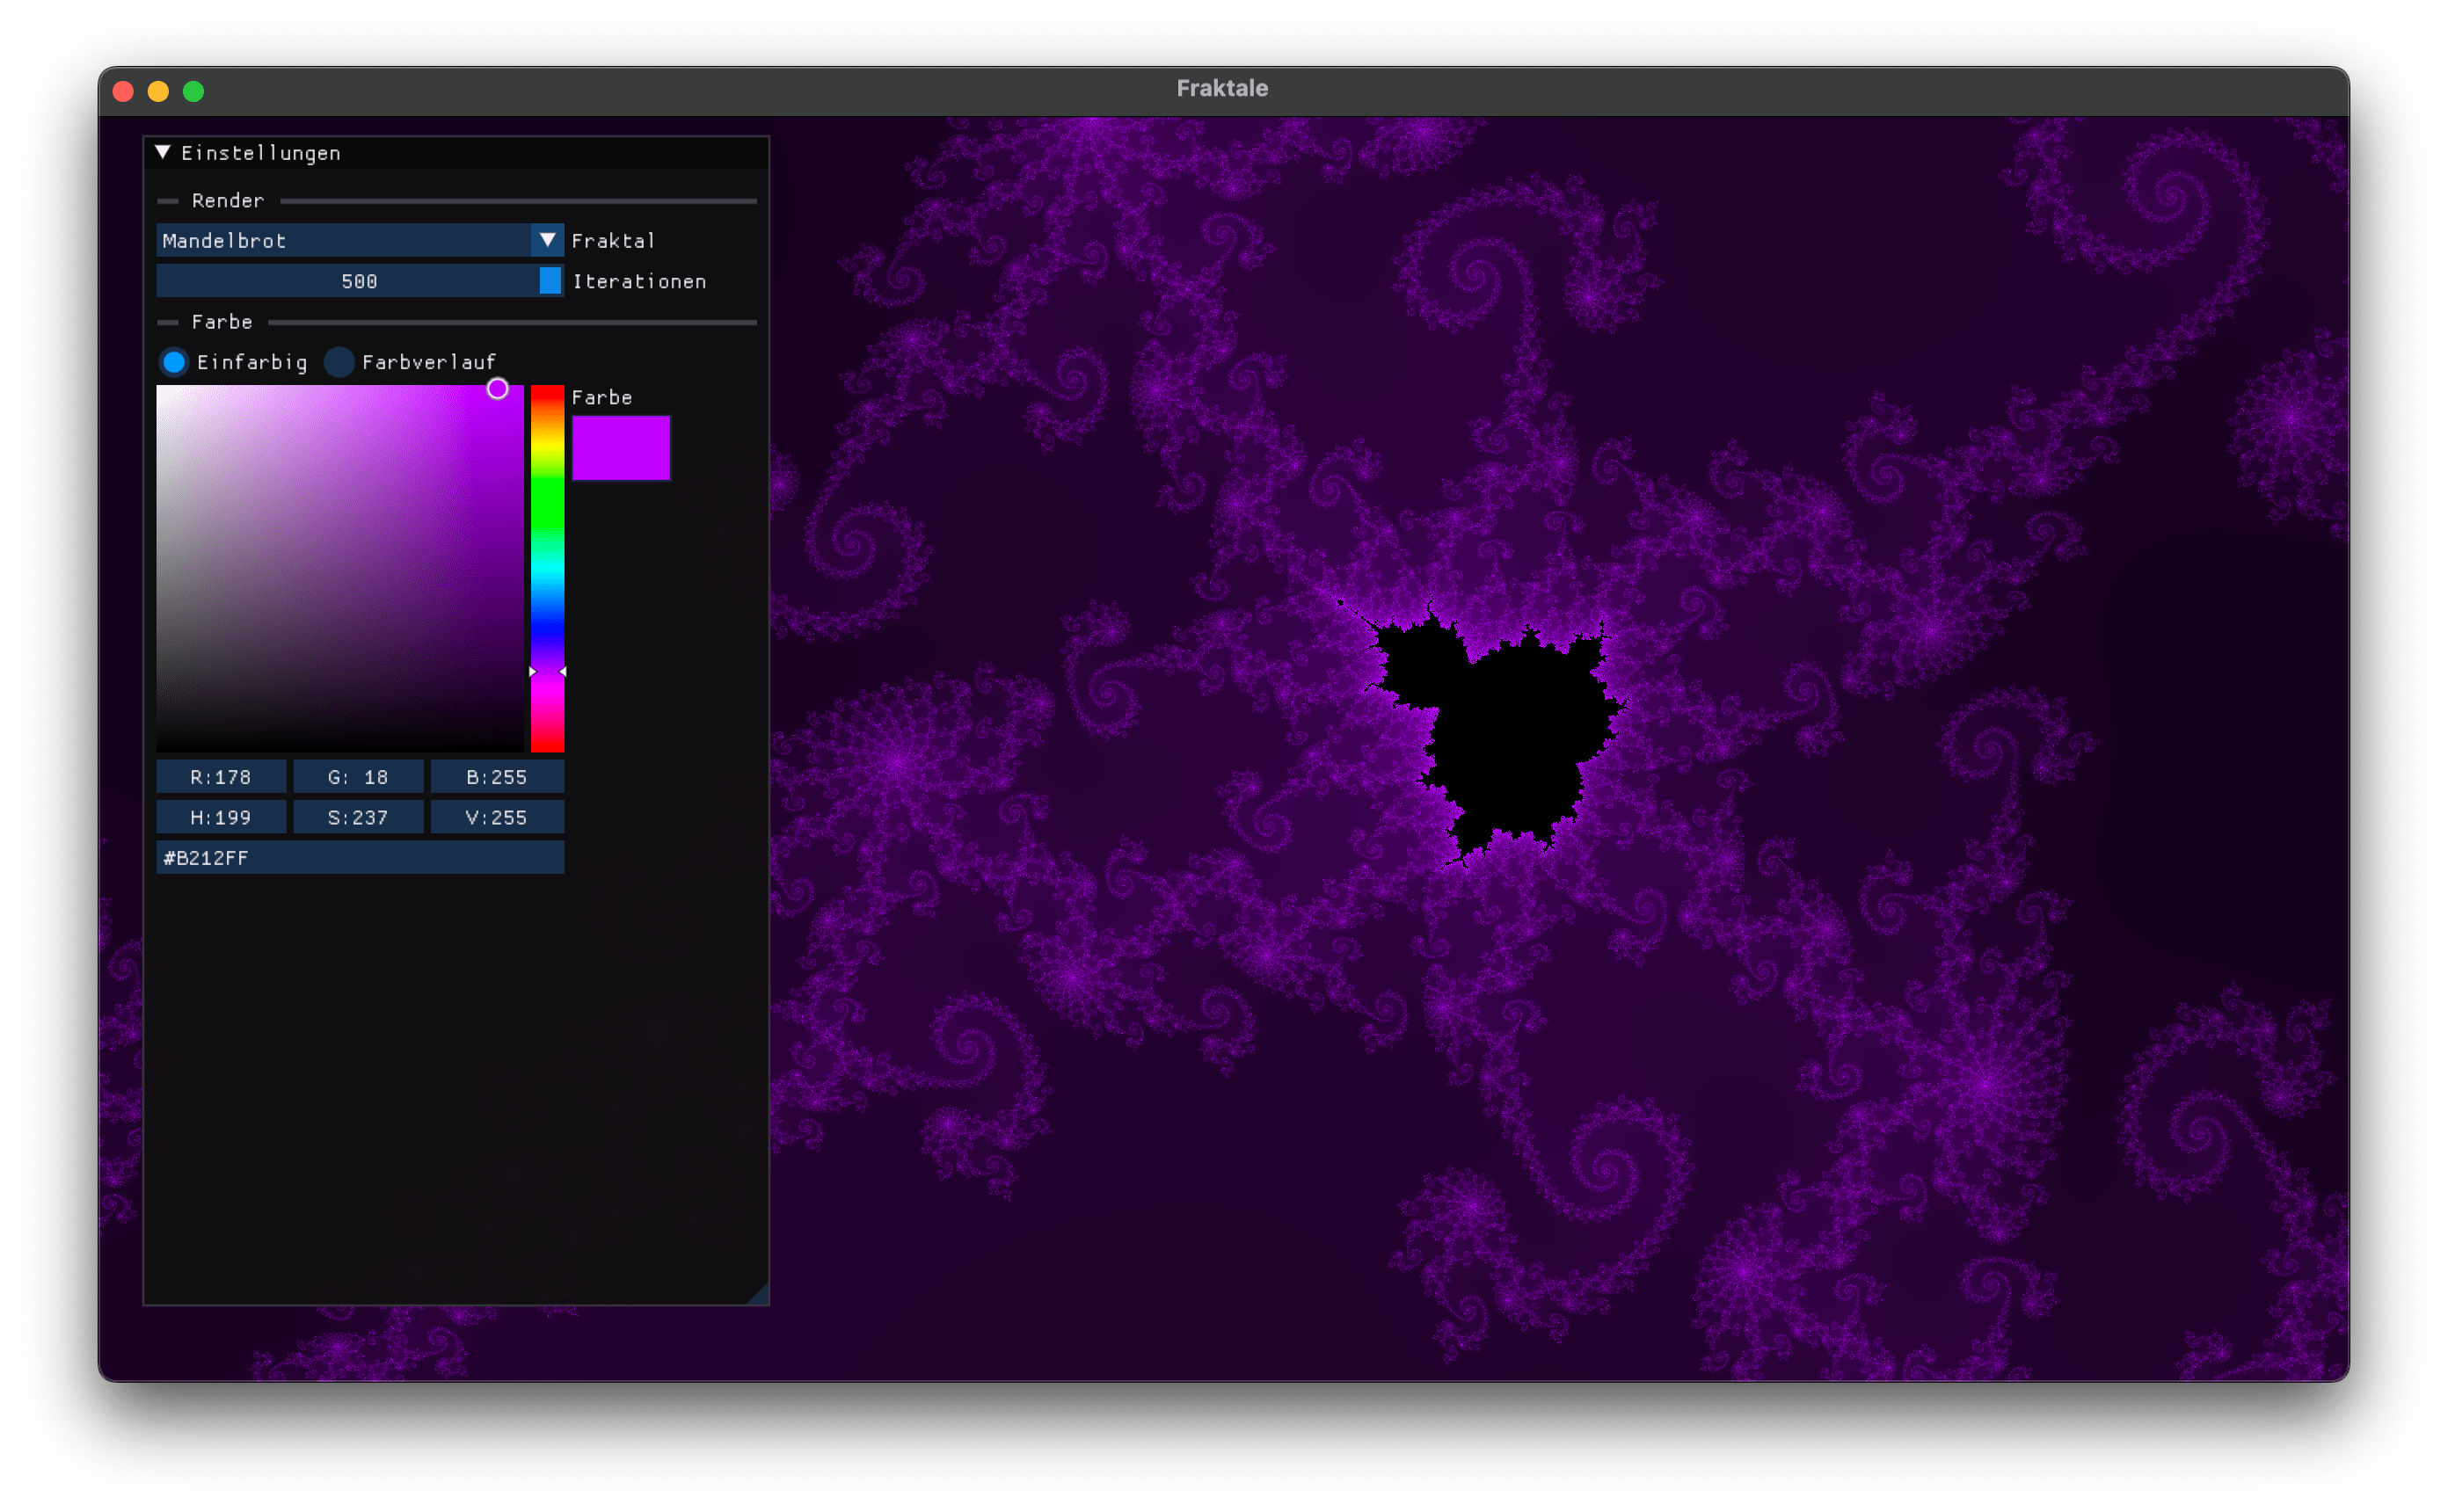
\includegraphics[width=\linewidth]{img/MandelbrotSingle.png}
%     \caption{\newline Mandelbrot-Menge mit \newline verschiedenen Lila-Tönen}\label{fig:mandelbrot-single}
%     \endminipage\hfill
%     \minipage{0.45\textwidth}
%     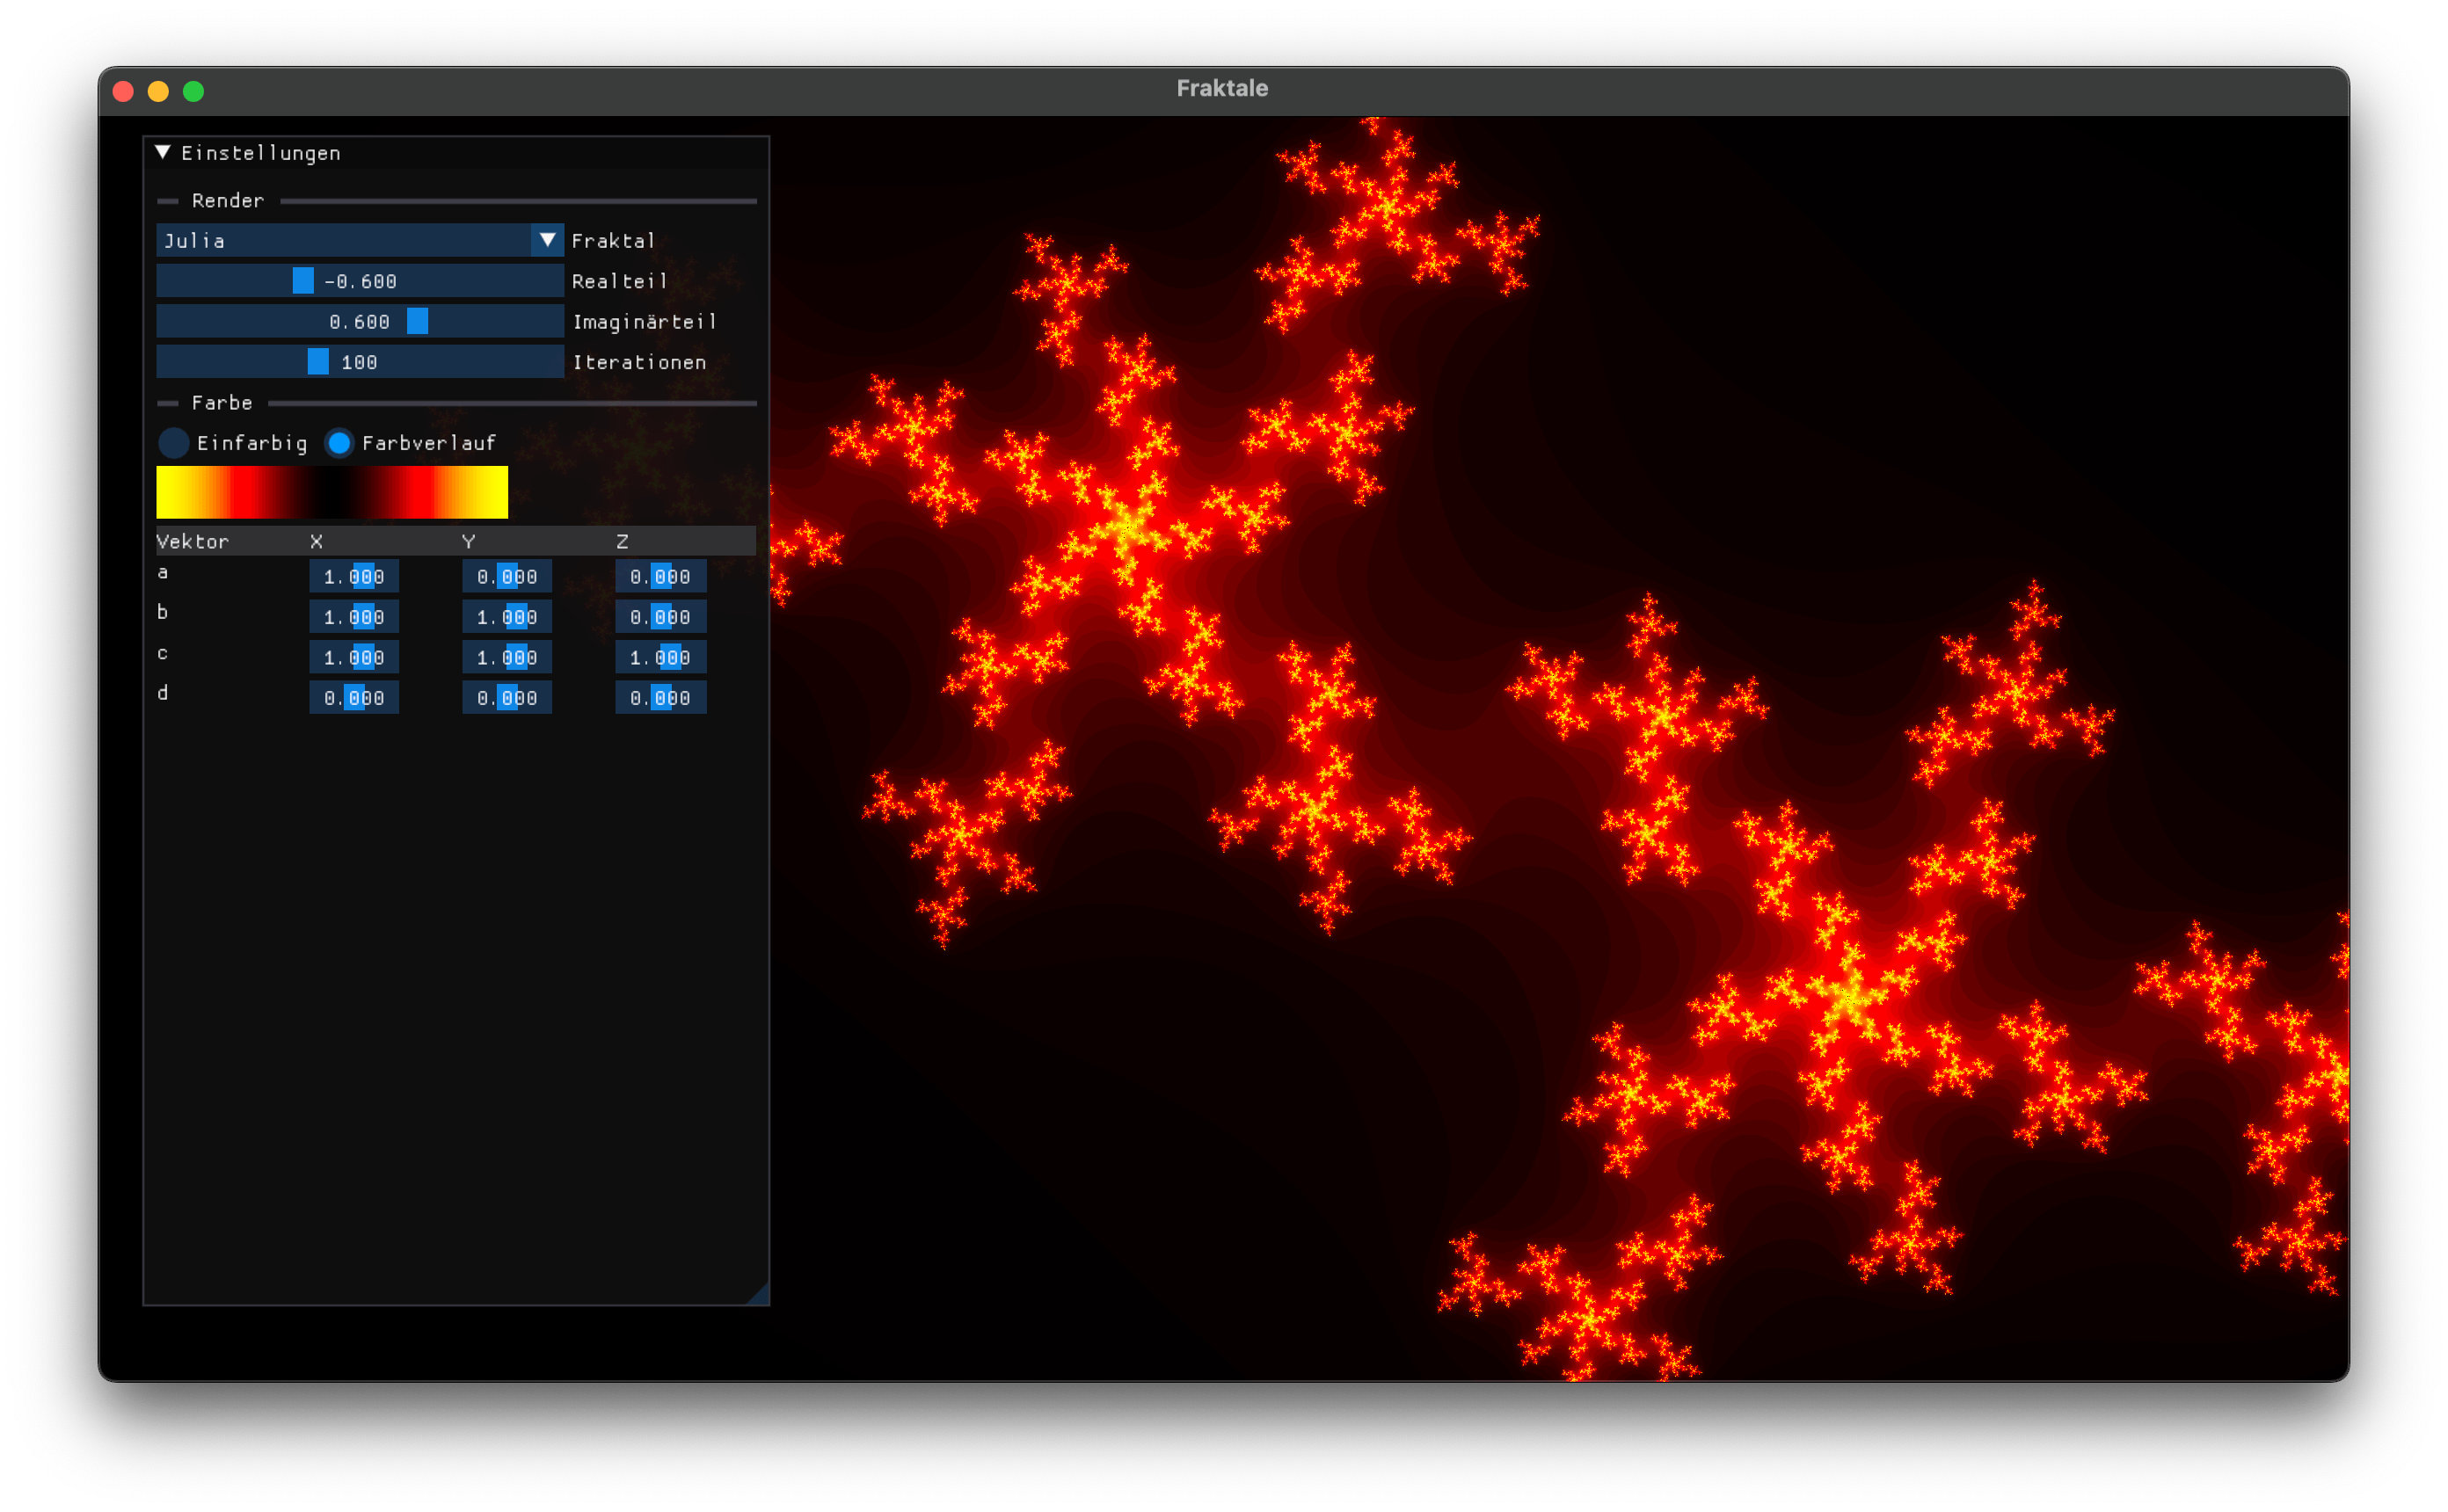
\includegraphics[width=\linewidth]{img/Julia-Red-Yellow.png}
%     \caption{\newline Julia-Menge für $c=-0.6+0.6i$ mit Gelb-Rot-Farbverlauf}\label{fig:julia-red-yellow}
%     \endminipage\hfill
% \end{figure}

\subsubsection{Einfarbig}
Die einfache Farbgebung erfolgt durch die Funktion \texttt{colorize\_single}.
\begin{verbatim} 
vec3 colorize_single(float n) {
    if(n == u_iterations) {
        return vec3(0.0, 0.0, 0.0);
    }
    float hue = n / u_iterations;
    return u_color * vec3(hue, hue, hue);
}
\end{verbatim}
Die Farbe wird durch einen \textit{RGB-Vektor} repräsentiert. Die vom Benutzer
eingestellte Farbe \texttt{u\_color} wird mit dem \texttt{hue}-Wert
multipliziert, der den Anteil der benötigten Iterationen zur Iterationsgrenze
darstellt.
\begin{figure}[H]
    \centering
    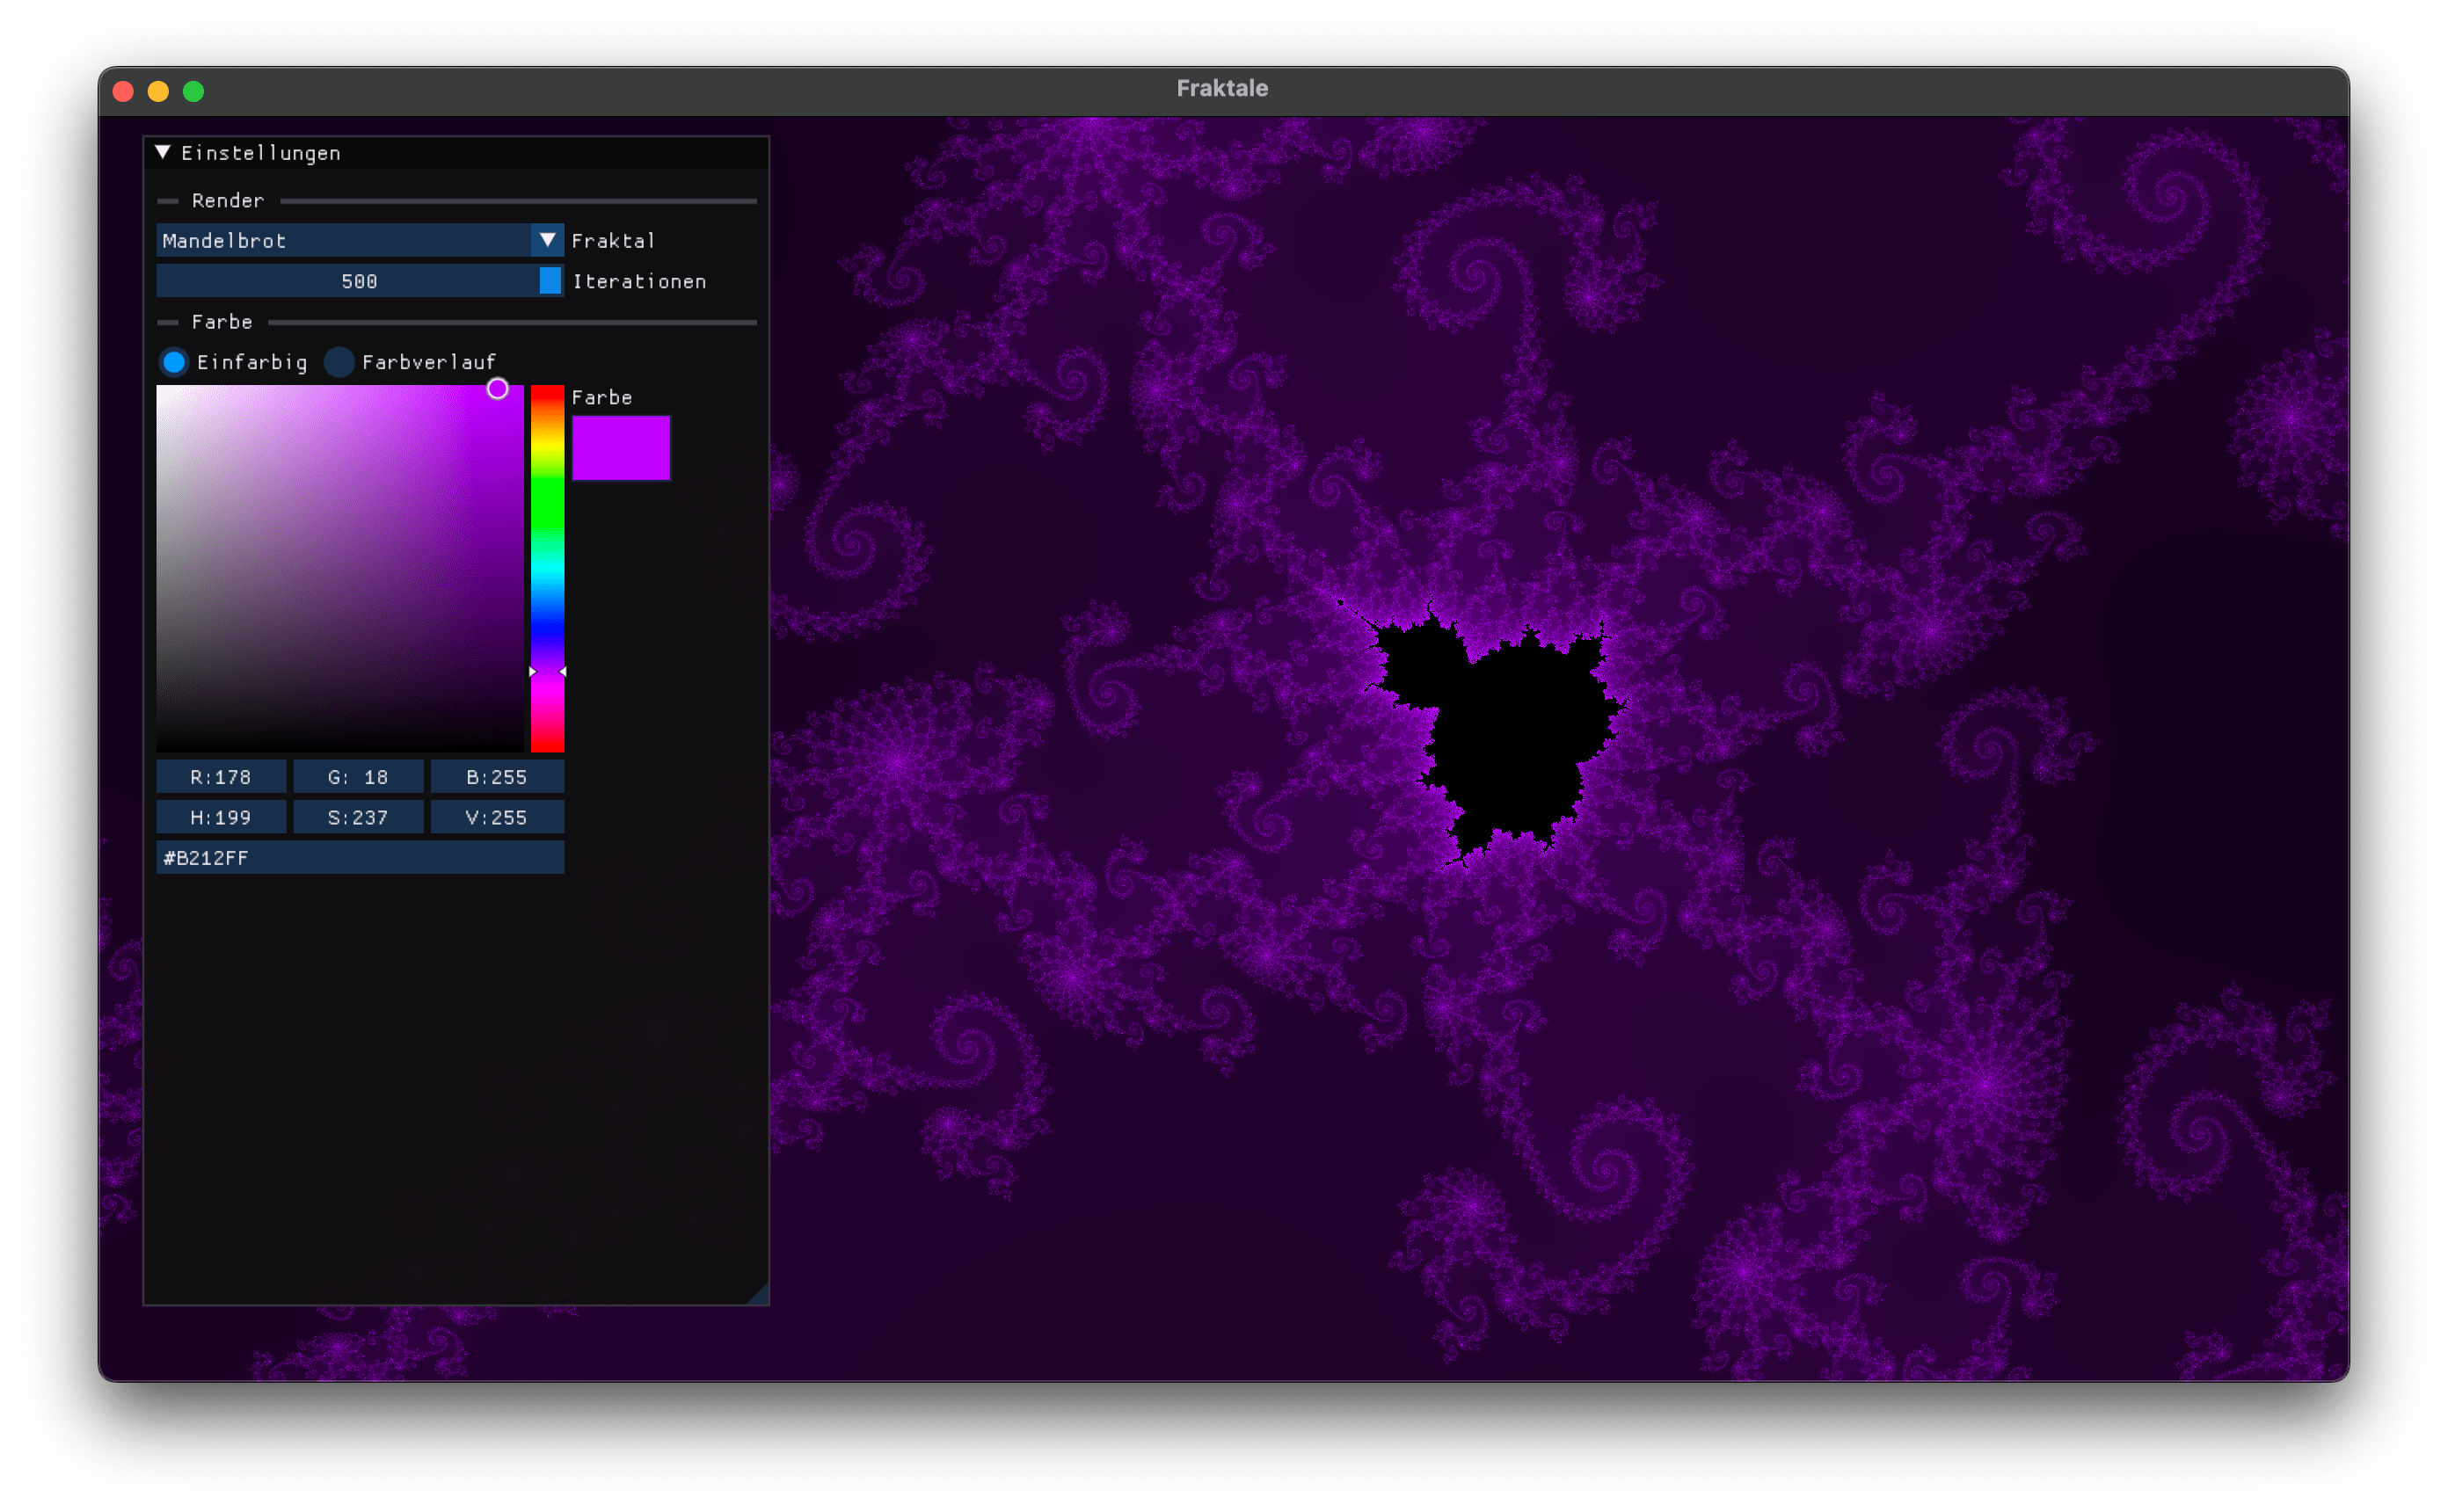
\includegraphics[width=0.75\textwidth]{img/MandelbrotSingle.png}
    \caption{Mandelbrot-Menge mit verschiedenen Lila-Tönen}
\end{figure}

\subsubsection{Farbverlauf}
Die Farbgebung mit Farbverlauf erfolgt durch die Funktion
\texttt{colorize\_gradient}.
\begin{verbatim}
vec3 colorize_gradient(float n) {
    if(n == u_iterations) {
        return vec3(0.0, 0.0, 0.0);
    }
    float t = n / u_iterations + 0.5;
    return u_a.xyz + u_b.xyz * cos(6.28318 * (u_c.xyz * t + u_d.xyz));
}
\end{verbatim}
\noindent
Die Funktion \texttt{colorize\_gradient} wird verwendet, um einen Farbverlauf basierend auf der Gleichung $f(t) = a + b \cdot \cos(2\pi(c \cdot t + d))$ \cite{InigoQui32:online} zu generieren. Hierbei handelt es sich um 3 Funktionen für die Farbwerte Rot, Grün und Blau mit 4 unterschiedlichen Parametern, wobei $a$, $b$, $c$ und $d$ RGB-Vektoren sind, die vom Benutzer festgelegt werden können.

\begin{figure}[H]
    \centering
    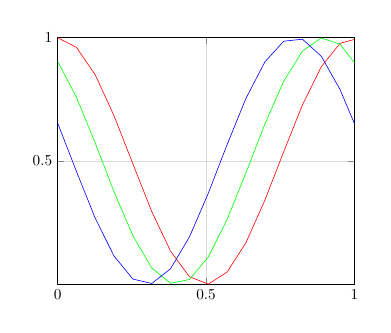
\begin{tikzpicture}[scale=0.55]
        \begin{axis}[
                xmin=0, xmax=1,
                ymin=0, ymax=1,
                xtick={0,0.5,1,2,3},
                ytick={1,0.5,2,3}, grid=both, minor tick num=1, major grid style={line
                        width=.2pt,draw=gray!30}, minor grid style={line width=.1pt,draw=gray!30}, ]

            % Function 1
            \addplot[
                domain=0:2*pi,
                samples=100,
                color=red,
            ] {0.5 + 0.5*cos(deg(2*pi*(1.0*x + 0.00)))};

            % Function 2
            \addplot[
                domain=0:2*pi,
                samples=100,
                color=green,
            ] {0.5 + 0.5*cos(deg(2*pi*(1.0*x + 0.10)))};

            % Function 3
            \addplot[
                domain=0:2*pi,
                samples=100,
                color=blue,
            ] {0.5 + 0.5*cos(deg(2*pi*(1.0*x + 0.20)))};

        \end{axis}
    \end{tikzpicture}
    \caption{Die entgültige Farbe wird durch die Addition der einzelnen Farbwerte für den Wert $t$ berechnet.}
\end{figure}
\noindent
\begin{figure}[H]
    \centering
    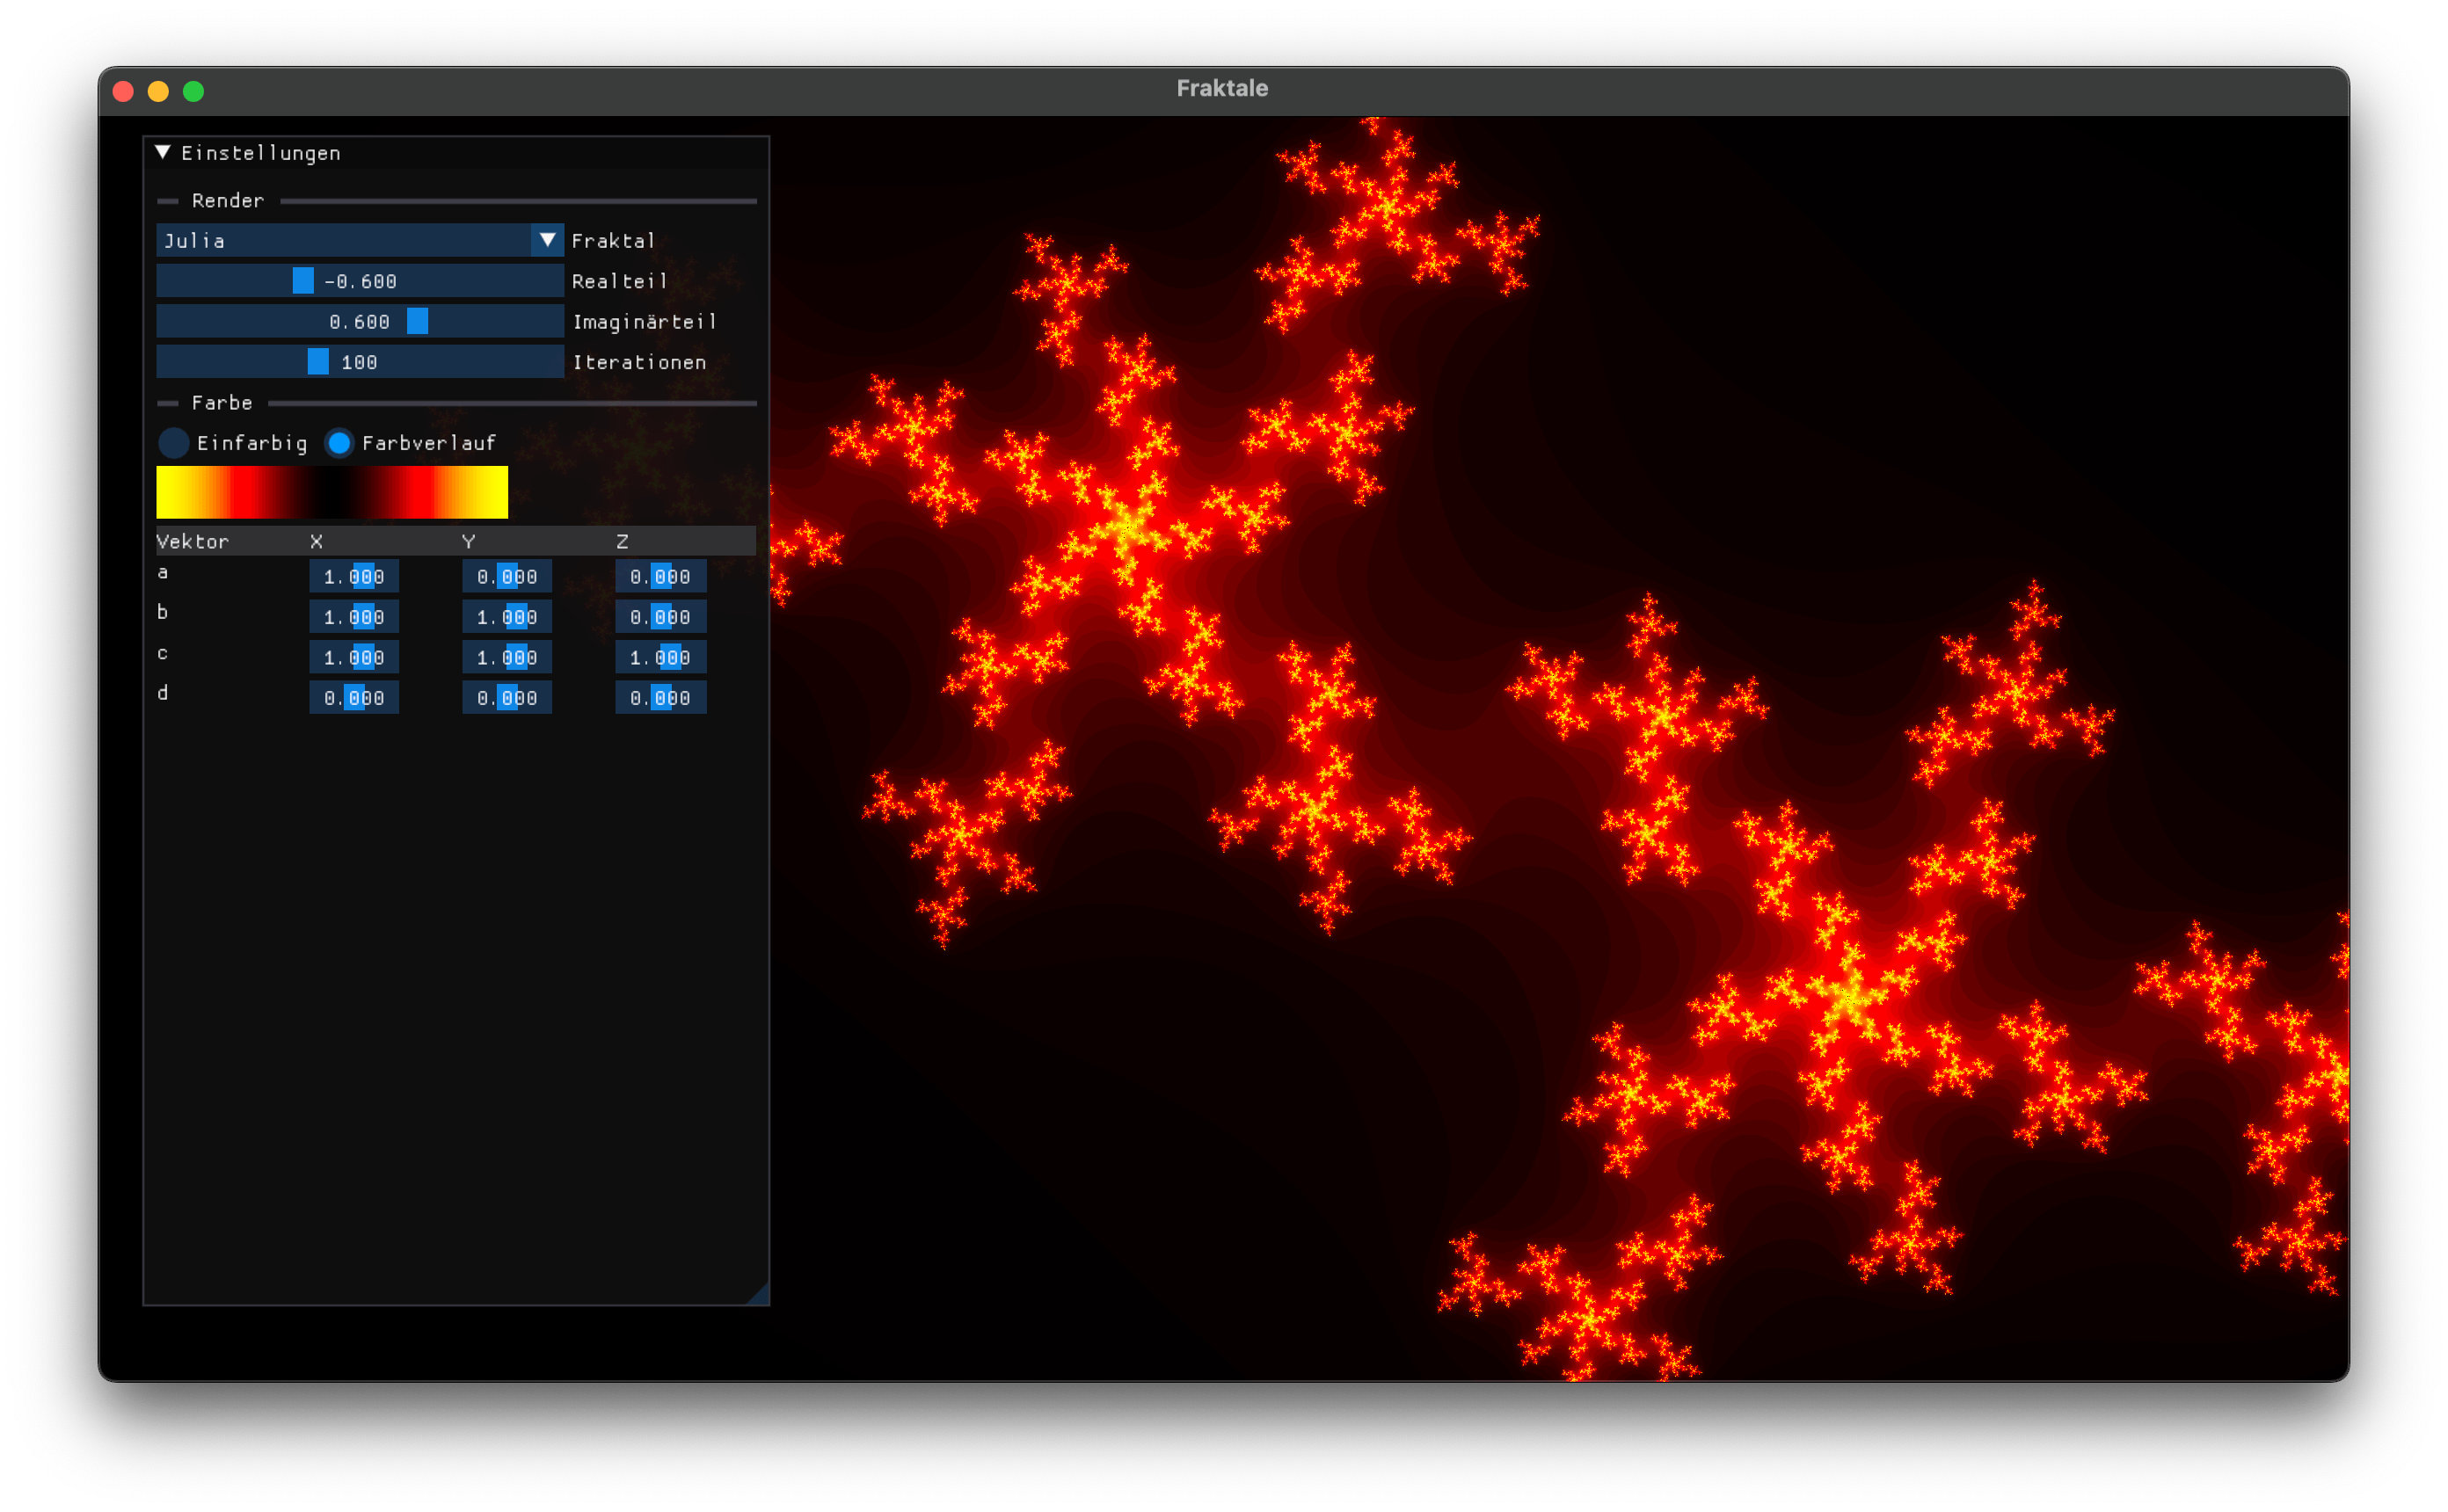
\includegraphics[width=0.75\textwidth]{img/Julia-Red-Yellow.png}
    \caption{Julia-Menge für $c=-0.6+0.6i$ mit Gelb-Rot-Farbverlauf}
\end{figure}